\section{Experimental details}
\label{app:experimental-details}

\subsection{Original audit inventory}

Table~\ref{tab:primary-audit-inventory} records the original audit units.  The three response checkpoints and three byte-LM decision checkpoints
are paired by training seed.  The ASLoRA runs are a separate RoBERTa-base/MRPC
experiment.

All numerical entries in the three original audit tables are generated directly from
\texttt{results/response\_summary.json},
\texttt{results/aslora\_summary.json}, and
\texttt{results/router\_decisions\_summary.json} by
\texttt{experiments/generate\_paper\_audit\_tables.py}.  Each generated file
records the SHA256 of its source summary, retaining negative seeds and failed
searches in the reported aggregates; the same script emits the appendix metric
and search-detail tables.  The additive tomography numbers are
generated separately from
\texttt{results/response\_tomography\_summary.json} by
\texttt{experiments/generate\_response\_tomography\_latex.py}; this leaves the
source-attested older response table unchanged.
The subsequent full-dimensional autodiff and factor-recovery tables are
generated by their separate summarizers from
\texttt{results/autograd\_tomography/} and
\texttt{results/factor\_recovery/}. Both validate generation-source and
checkpoint hashes. They reuse the same three checkpoints and therefore do
not increase the number of independent training seeds.

\begin{table}[H]
\centering
\small
\caption{Original primary audit inventory. Each audit has three seeds;
counts include failed searches and controls. Additive audits reuse the
response checkpoints, as detailed below.}
\label{tab:primary-audit-inventory}
\begin{tabular}{@{}p{.20\linewidth}p{.39\linewidth}p{.32\linewidth}@{}}
\toprule
Audit & Per-seed protocol & Required checks \\
\midrule
Optimizer response & 8 Gaussian and 4 designed probes; fixed non-permutation and permutation control & Rank, formula, exact-gauge product, reconstruction \\
ASLoRA first merge & 10 gauges; adjacent/all pairs and per-projection/joint actions & Coverage, canonical action, restoration \\
Byte-LM partition fold & 5,000 trials; four-group, same-effective refits & Fixed search and paired evaluation \\
\bottomrule
\end{tabular}
\end{table}

The response audit uses a fixed gauge strength of $0.35$, unit Euclidean
learning rates for both parameter blocks, and probe seeds determined before
evaluation.  Each result records its checkpoint and source hashes.  The best
finite-difference scale on a predeclared four-row, 32-coordinate checkpoint
extraction is selected only to validate the closed-form response; the eight
fixed Gaussian directions on the full $12\times787{,}712$ packed model provide
the separate non-permutation detection test.  The additive four-probe audit
constructs the Corollary~\ref{cor:response_tomography} design from \(\Theta\)
and reconstructs the response components.  Its full-dimensional responses are
evaluations of the already checked analytic formula, not four additional
full-model autograd/JVP calls.  Its version-2 artifacts separately record the
reference rank/dimension gate, the floating-point product residual, and exact
common-product validity from the explicit invertible-gauge construction.

The subsequent autodiff audit instead differentiates the packed factor map.
For each checkpoint it measures four designed and two unseen responses in
each of three charts: native, permutation, and a fixed non-permutation gauge.
Its five-level observation-noise diagnostic uses the native chart. The
factor-recovery pilot makes four fresh native-chart measurements, reuses one
fixed diagonalization weight seed across checkpoints, and reports all five
noise levels without selecting a favorable weight vector. True factors enter
the observation oracle and post-reconstruction error calculation, but not the
reconstruction routine. Neither experiment differentiates the language-model
task loss or simulates an AdamW trajectory.

The ASLoRA protocol follows the paper's defined configuration: 30 epochs,
effective batch size 16, rank eight, $\alpha=16$, $T_s=320$, and merge interval
240.  Appendix Table~5 of the source additionally records an update ratio
$\lambda=0.5$, but the accessible method text and Algorithm~1 define no
operation involving that quantity.  We record $\lambda$ as \texttt{update\_ratio\_record\_only}; the
reimplementation assigns it no operation because the source defines none.  With the one-indexed rule $t>T_s$ and
$(t-T_s)\bmod 240=0$, the first audit point is $t=560$.  Running $B$ is observed
after every optimizer update.  The three
artifacts contain 204, 208, and 200 canonical action evaluations, respectively:
all 66 query-only, 66 value-only, and 66 joint-same-pair actions plus every
additional composite selected by a declared baseline or gauge.  There are no
missing or undeclared candidates.  Every temporary tie is restored, the
trainable digest and parameter identities agree before and after the audit, and
no merge is committed.

The amendment chronology in
\texttt{research/ASLORA\_EMPIRICAL\_PROTOCOL.md} records the superseded
nondeterministic \(12/30\) and \(16/30\) batch, its source hashes, the
outcome-blind deterministic protocol lock, and the canonical replacement by
the \(11/30\) and \(14/30\) results reported here.

The ASLoRA artifacts contain two numerical paths. The primary path transforms the frozen running factors in float64, chooses a
layer-index action, and evaluates that action in the canonical model.  All
canonical gates pass.  The diagnostic path re-executes the live factorized
float32 model and also passes its tolerance in all three deterministic runs.
No main-paper metric is taken from that diagnostic path.  Both
candidate interpretations are retained because Algorithm~1 and the prose in
the source differ on whether all or only adjacent layer pairs are sorted.

% Auto-generated by experiments/generate_paper_audit_tables.py; do not edit.
% Source: results/aslora_summary.json
% Source SHA256: 1be80d31ca4208c414698c3b5fbd45bfb9d51835aa8f16f8cb43bab082840c41
\begin{table}[H]
\centering
\small
\caption{Canonical validation accuracy and F1 differences for the four ASLoRA candidate/scope cells in Table~\ref{tab:aslora-chain}.  Intervals range over all 30 selected gauge actions in each cell, including unchanged selections, and are selected-action minus identity-action differences.}
\label{tab:aslora-metric-details}
\begin{tabular}{@{}llcc@{}}
\toprule
Candidates & Scope & $\Delta$ accuracy & $\Delta$ F1 \\
\midrule
Adjacent & per-projection & $[-0.0025,+0.0098]$ & $[-0.0022,+0.0057]$ \\
Adjacent & joint pair & $[-0.0049,+0.0000]$ & $[-0.0051,+0.0000]$ \\
All pairs & per-projection & $[-0.0025,+0.0098]$ & $[-0.0022,+0.0057]$ \\
All pairs & joint pair & $[+0.0000,+0.0000]$ & $[+0.0000,+0.0000]$ \\
\bottomrule
\end{tabular}
\end{table}


% Auto-generated by experiments/generate_paper_audit_tables.py; do not edit.
% Source: results/aslora_summary.json
% Source SHA256: 1be80d31ca4208c414698c3b5fbd45bfb9d51835aa8f16f8cb43bab082840c41
\begin{table}[H]
\centering
\small
\caption{Declared alternatives for the primary per-projection ASLoRA decision.  Effective-update and local-activation rules are gauge invariant.  Their cells give the selected action and canonical validation-loss difference from the identity raw-$B$ action (negative is lower; exact zero is a tie).  Across the six rows, effective has 2 negative/2 positive/2 zero differences and local activation has 2 negative/1 positive/3 zero differences; neither rule uniformly improves across all seeds under both candidate readings.  Validation minima are separate query-only and value-only enumerations; they are not a full Cartesian per-projection oracle.}
\label{tab:aslora-baselines}
\setlength{\tabcolsep}{3pt}
\begin{tabular}{ccllll}
\toprule
Seed & Candidates & \shortstack[l]{Raw running $B$} & \shortstack[l]{Current effective} & \shortstack[l]{Local activation} & \shortstack[l]{Single-target\\minima} \\
\midrule
0 & Adjacent & \shortstack[l]{$Q:0\leftarrow1$\\$V:0\leftarrow1$} & \shortstack[l]{$Q:0\leftarrow1$\\$V:10\leftarrow11$\\$\Delta L=-0.0336$} & \shortstack[l]{$Q:0\leftarrow1$\\$V:0\leftarrow1$\\$\Delta L=+0.0000$} & \shortstack[l]{$Q:6\leftarrow7$\\$V:10\leftarrow11$} \\
0 & All pairs & \shortstack[l]{$Q:0\leftarrow1$\\$V:0\leftarrow1$} & \shortstack[l]{$Q:0\leftarrow1$\\$V:1\leftarrow11$\\$\Delta L=-0.0075$} & \shortstack[l]{$Q:0\leftarrow1$\\$V:0\leftarrow11$\\$\Delta L=-0.0008$} & \shortstack[l]{$Q:6\leftarrow9$\\$V:10\leftarrow11$} \\
1 & Adjacent & \shortstack[l]{$Q:0\leftarrow1$\\$V:2\leftarrow3$} & \shortstack[l]{$Q:0\leftarrow1$\\$V:10\leftarrow11$\\$\Delta L=+0.0018$} & \shortstack[l]{$Q:0\leftarrow1$\\$V:0\leftarrow1$\\$\Delta L=+0.0001$} & \shortstack[l]{$Q:4\leftarrow5$\\$V:3\leftarrow4$} \\
1 & All pairs & \shortstack[l]{$Q:0\leftarrow2$\\$V:0\leftarrow2$} & \shortstack[l]{$Q:0\leftarrow3$\\$V:10\leftarrow11$\\$\Delta L=+0.0028$} & \shortstack[l]{$Q:0\leftarrow3$\\$V:0\leftarrow11$\\$\Delta L=-0.0005$} & \shortstack[l]{$Q:4\leftarrow11$\\$V:3\leftarrow5$} \\
2 & Adjacent & \shortstack[l]{$Q:0\leftarrow1$\\$V:0\leftarrow1$} & \shortstack[l]{$Q:0\leftarrow1$\\$V:0\leftarrow1$\\$\Delta L=+0.0000$} & \shortstack[l]{$Q:0\leftarrow1$\\$V:0\leftarrow1$\\$\Delta L=+0.0000$} & \shortstack[l]{$Q:8\leftarrow9$\\$V:8\leftarrow9$} \\
2 & All pairs & \shortstack[l]{$Q:0\leftarrow1$\\$V:0\leftarrow1$} & \shortstack[l]{$Q:0\leftarrow1$\\$V:0\leftarrow1$\\$\Delta L=+0.0000$} & \shortstack[l]{$Q:0\leftarrow1$\\$V:0\leftarrow1$\\$\Delta L=+0.0000$} & \shortstack[l]{$Q:8\leftarrow11$\\$V:8\leftarrow11$} \\
\bottomrule
\end{tabular}
\end{table}


The byte-LM search makes 5,000 predeclared positive-stochastic trials per
checkpoint and preserves a four-group action budget.  Failed searches retain
their attempted, invertible, condition-passing, simplex-passing, and
group-passing counts.  The successful contrast refits both partitions from
common effective tensors.  Literal hardening is excluded from the primary
comparison because it changes basis coordinates and the partition jointly.
All three routers satisfy the initialization-dominated flag.  Only seed 0
reaches decision evaluation: its k-means and Ward effective-tensor baselines
both have BPB $2.1753145$ and centroid SSE $5.46896\times10^{-5}$.  Seeds 1 and
2 store no folds or baseline evaluation because their searches exit first.
Signed-local and same-sorted-group-size searches were not executed in that
historical audit; they were
post-run, non-primary protocol amendments.  In particular, the observed
group-size change $3/3/3/3\to5/3/3/1$ remains a balance confound.
The reported interval resamples the 256 paired evaluation-batch differences
10,000 times. It describes evaluation variability conditional on this
checkpoint and selected contrast; it does not cover training-seed or
gauge-search uncertainty.

The protocol defines the initialization-dominated flag as mean row-wise router
$L_1$ movement from initialization strictly below $0.01$.  The three observed
movements round to $0.000313$--$0.000401$, so every checkpoint meets that
declared threshold; this flag describes training movement, not recovery of a
historical graph.

% Auto-generated by experiments/generate_paper_audit_tables.py; do not edit.
% Source: results/router_decisions_summary.json
% Source SHA256: 0e863e1db624a7f25697a7a6873e83e91f928458ba61cdfd06081e582b3e28f2
\begin{table}[H]
\centering
\small
\setlength{\tabcolsep}{4pt}
\caption{Byte-LM checkpoint and finite-search diagnostics omitted from the compact main table.  The funnel is attempted/invertible/condition-pass/simplex-pass/group-pass/partition-change.}
\label{tab:router-search-details}
\begin{tabular}{@{}crrc@{}}
\toprule
Seed & Soft BPB & Mean row router $L_1$ move & Search funnel A/I/C/S/G/P \\
\midrule
0 & 2.186 & $3.35\!\times\!10^{-4}$ & 5000/5000/4586/4586/3762/1 \\
1 & 2.188 & $3.13\!\times\!10^{-4}$ & 5000/5000/4601/4601/3790/0 \\
2 & 2.168 & $4.01\!\times\!10^{-4}$ & 5000/5000/4581/4581/3769/0 \\
\bottomrule
\end{tabular}
\end{table}

\begin{table}[H]
\centering
\small
\setlength{\tabcolsep}{3pt}
\caption{Geometry and gauge-invariant comparator details for the sole completed byte-LM witness.  The k-means and Ward folds coincide here; the unigram baseline is included only as a scale reference.}
\label{tab:router-witness-details}
\begin{tabular}{@{}crccccr@{}}
\toprule
Seed & $\kappa(Q)$ & Group sizes ref.$\to$cand. & Disagreement & k-means/Ward BPB & Centroid SSE & Unigram BPB \\
\midrule
0 & 7.93 & 3/3/3/3$\to$5/3/3/1 & 0.121 & 2.175/2.175 & $5.47\!\times\!10^{-5}$ & 4.624 \\
\bottomrule
\end{tabular}
\end{table}


\section{Secondary planted-data and probe sanity checks}
\label{app:secondary-sanity}

The original \TyingBench{} and \method{} experiments below check the
implementation and illustrate the theory in planted settings. They are
secondary to the main experiments and do not estimate the prevalence of
router misinterpretation in deployed systems.

\subsection{\TyingBench{} protocols}

\paragraph{Exact factorization.}
We generate $K$ orthogonal basis vectors with controlled condition number,
choose one of five depth graphs (cycle, contiguous, palindrome, balanced
random, or imbalanced), and expose the resulting effective layer vectors.  We
jointly fit soft bases and router coefficients from neutral, random,
correct-pattern, and deliberately wrong-pattern initializations.  Hard
straight-through, vertex-regularized, $k$-means, and oracle estimators provide
comparisons.  This setting removes sampling error: failure is factorization or
optimization ambiguity, not insufficient task data.

\paragraph{Functional distillation.}
A planted one-hot teacher and a jointly trained soft student share the same
architecture and basis budget.  We use an eight-layer residual MLP and an
eight-layer decoder-only Transformer.  The Transformer mixes parameters before
applying each block, evaluates one block per layer, and uses an explicit
upper-triangular causal mask.  Students observe teacher outputs but not the
teacher graph.  Test MSE or KL measures function fit; ARI measures recovery of
the planted graph.  These labels are legitimate for the planted teacher, not
for the natural-language experiment.

\paragraph{Language-model stability arm.}
We train a 12-layer, four-basis causal Transformer on WikiText-2 bytes.  The
task has no privileged sharing graph, so this arm has no recovery label.  BPB,
router movement, and cross-run graph agreement diagnose path dependence only.
It is separate from the original same-budget partition-fold audit.

\begin{table}[H]
\centering
\scriptsize
\caption{Secondary sanity-sweep sizes.  Every listed seed is crossed with the
conditions defined by the corresponding executable sweep.}
\label{tab:sweep-configs}
\begin{tabular}{lrrrrl}
\toprule
Family & Depth & Bases & Width & Seeds & Budget / grid \\
\midrule
Factorization & 12 & 4 & 128 & 10 & 2,000 steps; 5 graphs \\
Residual MLP distillation & 8 & 4 & 64 & 5 & 1,500 steps; 4 graphs \\
Causal Transformer distillation & 8 & 4 & 64 & 5 & 1,000 steps; 4 graphs \\
Functional probes & 12 & 4 & 64 & 10 & $n\in\{1,2,4,8,16,32,64\}$; 6 noise levels \\
WikiText-2 stability & 12 & 4 & 256 & 3 & 1,500 steps; context 128 \\
\bottomrule
\end{tabular}
\end{table}

All models use parameter-space mixing: each effective tensor is formed once
from the same layer router row, and each block is evaluated once.  This avoids
the compute mismatch of an output-space mixture that evaluates all $K$ basis
blocks.  Teacher graphs and datasets are deterministic functions of recorded
seeds.  The causal Transformer test changes future tokens while asserting that
all earlier logits are unchanged.

\subsection{\method{} as a conditional diagnostic}

Native activations can confound a layer transition with the distribution
created by preceding layers.  \method{} draws
$H_1,\ldots,H_n\sim P_H$ once and evaluates every residual transition $r_\ell$
on the same inputs.  In the revised paired protocol, observations satisfy
$Y_{\ell s}=r_\ell(H_s)+\sigma\epsilon_{\ell s}$ with iid standard-Gaussian
noise at a fixed absolute scale $\sigma$.  Its signature and empirical squared
distance are
\begin{equation}
  \phi_\ell=n^{-1/2}[Y_{\ell1};\ldots;Y_{\ell n}],\qquad
  \widehat d_{\ell m}^2=\|\phi_\ell-\phi_m\|_2^2.
  \label{eq:shareprobe}
\end{equation}
Counterfactual and native estimators use the same initial probes, noise array,
and optional random projection.  The native trajectory advances only with
clean residual updates.  Thus each method has the stated marginal observation
model and their difference uses common random numbers; unlike the superseded
implementation, noise is not rescaled by a realized batch standard deviation.
For example, layers using $f(h)=h$ and $g(h)=-h$ in the true pattern
$(f,g,f,g)$ yield the wrong native-output groups
$\{1,2\}\mid\{3,4\}$ on inputs $(1,-1,-1,1)$, whereas the common input $h=1$
recovers $\{1,3\}\mid\{2,4\}$.  This is a counterexample to an unqualified
native-trajectory interpretation, not evidence that native signatures are
generally inferior.

Table~\ref{tab:probes} shows no consistent empirical advantage for
\method{}.  Shared-input versus native mean ARI is $0.6764$ versus $0.6751$
for the MLP and $0.5006$ versus $0.5009$ for the Transformer.  The paired
win/tie/loss counts are $65/1570/45$ and $61/1558/61$, respectively, and the
seed-averaged difference changes sign (six of ten MLP seeds but only three of
ten Transformer seeds favor shared inputs).  A simple baseline clusters the
concatenated visible effective weights and biases of every mixed linear module;
it obtains ARI $1.000$ in every planted cell.  That baseline requires parameter
access and parameter distance is \emph{not} functional equivalence in a neural
network with parameter symmetries.  It nevertheless shows that the probe is
unnecessary in this benchmark when effective block tensors are visible.

We therefore retain \method{} only as a conditional functional diagnostic.
Its graph is invariant to factor coordinates and targets equivalence on
$P_H$, but the probe distribution must cover the claimed domain, $K$ must be
supplied to the clusterer, and the observed planted-partition gap becomes a
certificate only under the population-separation and uniform-tail assumptions
of Appendix~\ref{app:probe_proof}.  The experiment does not estimate those
population quantities.

\section{Secondary sanity results}

\IfFileExists{figures/gauge_equivalence.pdf}{%
\begin{figure}[H]
  \centering
  \begin{subfigure}[t]{.48\linewidth}
    \centering
    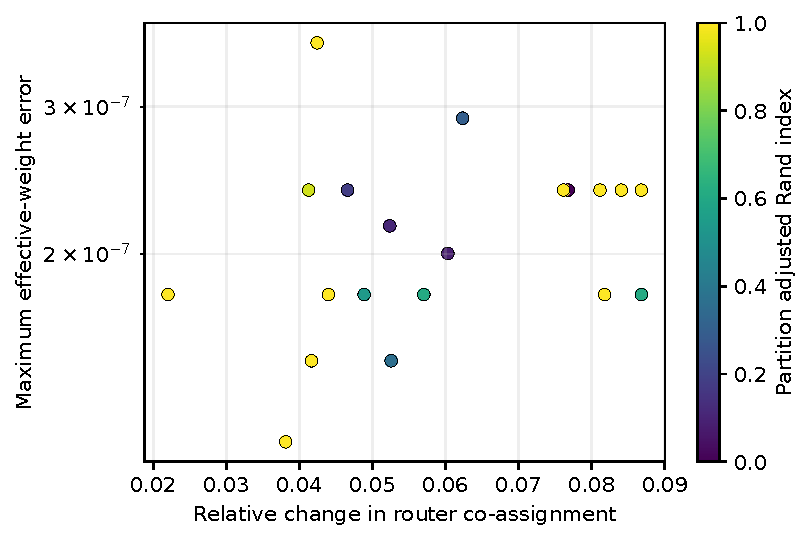
\includegraphics[width=\linewidth]{figures/gauge_equivalence.pdf}
    \caption{Gauge-equivalent routers.}
  \end{subfigure}\hfill
  \begin{subfigure}[t]{.48\linewidth}
    \centering
    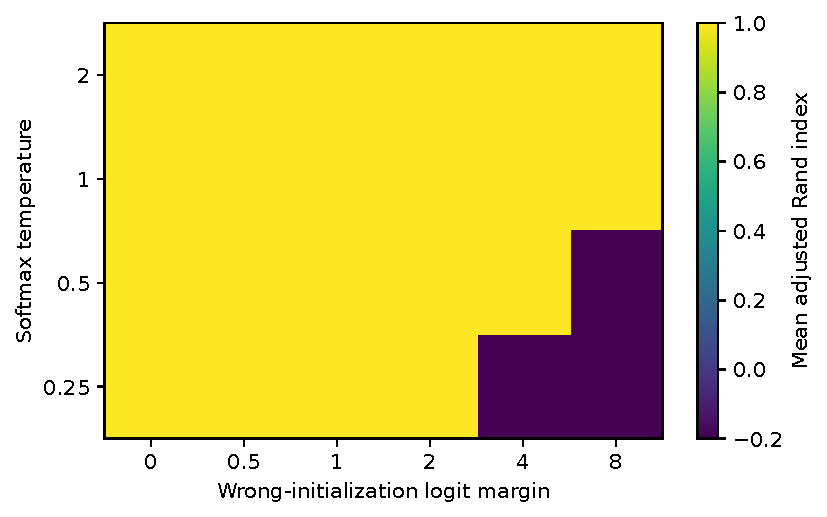
\includegraphics[width=\linewidth]{figures/saturation_recovery.pdf}
    \caption{Recovery from a wrong router.}
  \end{subfigure}
  \caption{Synthetic theory checks.  Effective weights remain equal at
  numerical precision while router summaries can change; saturation can
  suppress recovery from a deliberately wrong initialization.}
  \label{fig:gauge-saturation}
\end{figure}
}{}

The exact-factorization and distillation sweeps show that, for the tested
planted teachers and budgets, similar reconstruction or task loss need not
select the same router graph.  They are possibility and path-dependence checks,
not estimates of real-world frequency.  Discrete clustering succeeds when its
one-hot model matches the teacher, which is a positive control rather than a
general recovery guarantee.

\IfFileExists{generated/gauge_table.tex}{% Auto-generated by experiments/analyze_results.py; do not edit by hand.
\begin{table}[H]
\centering
\small
\caption{Gauge counterfactuals. Values are mean $\pm$ sample standard deviation across trials.}
\label{tab:gauge}
\begin{tabular}{lrr}
\toprule
Metric & Value & $n$ \\
\midrule
Effective max error & $2.11\!\times\!10^{-7} \pm 5.41\!\times\!10^{-8}$ & 20 \\
Argmax-partition ARI & $0.686 \pm 0.380$ & 20 \\
Co-assignment relative change & $0.059 \pm 0.019$ & 20 \\
Post-step effective relative difference & $0.002 \pm 9.90\!\times\!10^{-4}$ & 20 \\
\bottomrule
\end{tabular}
\end{table}
}{}
\IfFileExists{generated/saturation_table.tex}{% Auto-generated by experiments/analyze_results.py; do not edit by hand.
\begin{table}[H]
\centering
\scriptsize
\caption{Softmax-saturation sweep. Values are aggregated across seeds for each temperature and wrong-initialization margin.}
\label{tab:saturation}
\begin{tabular}{rrrrrr}
\toprule
Temperature & Margin & Initial grad. & Final MSE & ARI & $n$ \\
\midrule
0.250 & 0 & $0.008 \pm 4.18\!\times\!10^{-5}$ & $8.07\!\times\!10^{-8} \pm 2.96\!\times\!10^{-10}$ & $1.000 \pm 0$ & 5 \\
0.250 & 0.500 & $0.002 \pm 1.04\!\times\!10^{-10}$ & $7.88\!\times\!10^{-8} \pm 2.08\!\times\!10^{-13}$ & $1.000 \pm 0$ & 5 \\
0.250 & 1.000 & $4.62\!\times\!10^{-5} \pm 1.63\!\times\!10^{-12}$ & $6.00\!\times\!10^{-8} \pm 1.86\!\times\!10^{-13}$ & $1.000 \pm 0$ & 5 \\
0.250 & 2.000 & $1.55\!\times\!10^{-8} \pm 7.94\!\times\!10^{-16}$ & $1.94\!\times\!10^{-8} \pm 9.27\!\times\!10^{-14}$ & $1.000 \pm 0$ & 5 \\
0.250 & 4.000 & $9.14\!\times\!10^{-16} \pm 1.16\!\times\!10^{-22}$ & $0.021 \pm 2.28\!\times\!10^{-9}$ & $-0.222 \pm 3.10\!\times\!10^{-17}$ & 5 \\
0.250 & 8.000 & $0 \pm 0$ & $0.021 \pm 2.28\!\times\!10^{-9}$ & $-0.222 \pm 3.10\!\times\!10^{-17}$ & 5 \\
0.500 & 0 & $0.004 \pm 8.64\!\times\!10^{-6}$ & $2.52\!\times\!10^{-7} \pm 6.31\!\times\!10^{-10}$ & $1.000 \pm 0$ & 5 \\
0.500 & 0.500 & $0.004 \pm 2.65\!\times\!10^{-10}$ & $2.68\!\times\!10^{-7} \pm 4.13\!\times\!10^{-13}$ & $1.000 \pm 0$ & 5 \\
0.500 & 1.000 & $0.001 \pm 5.21\!\times\!10^{-11}$ & $2.76\!\times\!10^{-7} \pm 2.96\!\times\!10^{-13}$ & $1.000 \pm 0$ & 5 \\
0.500 & 2.000 & $2.31\!\times\!10^{-5} \pm 8.13\!\times\!10^{-13}$ & $2.49\!\times\!10^{-7} \pm 3.02\!\times\!10^{-13}$ & $1.000 \pm 0$ & 5 \\
0.500 & 4.000 & $7.74\!\times\!10^{-9} \pm 3.97\!\times\!10^{-16}$ & $1.44\!\times\!10^{-7} \pm 9.62\!\times\!10^{-14}$ & $1.000 \pm 0$ & 5 \\
0.500 & 8.000 & $4.57\!\times\!10^{-16} \pm 5.80\!\times\!10^{-23}$ & $0.021 \pm 2.28\!\times\!10^{-9}$ & $-0.222 \pm 3.10\!\times\!10^{-17}$ & 5 \\
1.000 & 0 & $0.002 \pm 1.73\!\times\!10^{-6}$ & $7.25\!\times\!10^{-7} \pm 7.43\!\times\!10^{-10}$ & $1.000 \pm 0$ & 5 \\
1.000 & 0.500 & $0.002 \pm 2.85\!\times\!10^{-10}$ & $7.17\!\times\!10^{-7} \pm 4.67\!\times\!10^{-13}$ & $1.000 \pm 0$ & 5 \\
1.000 & 1.000 & $0.002 \pm 1.33\!\times\!10^{-10}$ & $7.58\!\times\!10^{-7} \pm 5.92\!\times\!10^{-13}$ & $1.000 \pm 0$ & 5 \\
1.000 & 2.000 & $5.41\!\times\!10^{-4} \pm 2.60\!\times\!10^{-11}$ & $7.66\!\times\!10^{-7} \pm 3.52\!\times\!10^{-13}$ & $1.000 \pm 0$ & 5 \\
1.000 & 4.000 & $1.16\!\times\!10^{-5} \pm 4.07\!\times\!10^{-13}$ & $6.68\!\times\!10^{-7} \pm 6.33\!\times\!10^{-13}$ & $1.000 \pm 0$ & 5 \\
1.000 & 8.000 & $3.87\!\times\!10^{-9} \pm 1.99\!\times\!10^{-16}$ & $4.91\!\times\!10^{-7} \pm 1.19\!\times\!10^{-12}$ & $1.000 \pm 0$ & 5 \\
2.000 & 0 & $9.76\!\times\!10^{-4} \pm 1.81\!\times\!10^{-7}$ & $2.13\!\times\!10^{-6} \pm 4.74\!\times\!10^{-10}$ & $1.000 \pm 0$ & 5 \\
2.000 & 0.500 & $9.90\!\times\!10^{-4} \pm 8.23\!\times\!10^{-11}$ & $2.10\!\times\!10^{-6} \pm 1.15\!\times\!10^{-12}$ & $1.000 \pm 0$ & 5 \\
2.000 & 1.000 & $0.001 \pm 1.43\!\times\!10^{-10}$ & $2.09\!\times\!10^{-6} \pm 1.19\!\times\!10^{-12}$ & $1.000 \pm 0$ & 5 \\
2.000 & 2.000 & $9.09\!\times\!10^{-4} \pm 6.64\!\times\!10^{-11}$ & $2.19\!\times\!10^{-6} \pm 2.68\!\times\!10^{-12}$ & $1.000 \pm 0$ & 5 \\
2.000 & 4.000 & $2.71\!\times\!10^{-4} \pm 1.30\!\times\!10^{-11}$ & $2.17\!\times\!10^{-6} \pm 3.48\!\times\!10^{-12}$ & $1.000 \pm 0$ & 5 \\
2.000 & 8.000 & $5.78\!\times\!10^{-6} \pm 2.03\!\times\!10^{-13}$ & $1.82\!\times\!10^{-6} \pm 9.90\!\times\!10^{-13}$ & $1.000 \pm 0$ & 5 \\
\bottomrule
\end{tabular}
\end{table}
}{}
\IfFileExists{generated/factorization_full_table.tex}{%
  % Auto-generated by experiments/analyze_results.py; do not edit by hand.
\begin{table}[H]
\centering
\scriptsize
\caption{Exact-factorization results for cycle teachers. Values are mean $\pm$ sample standard deviation across seeds.}
\label{tab:factorization-full}
\resizebox{\linewidth}{!}{%
\begin{tabular}{lllrrrr}
\toprule
Method & Init relation & Raw init & Rel.\ error & ARI & Assignment acc. & $n$ \\
\midrule
k-means & neutral & neutral & $0 \pm 0$ & $1.000 \pm 0$ & $1.000 \pm 0$ & 10 \\
oracle & neutral & neutral & $0 \pm 0$ & $1.000 \pm 0$ & $1.000 \pm 0$ & 10 \\
soft & matched & cycle & $0.003 \pm 8.36\!\times\!10^{-4}$ & $1.000 \pm 0$ & $1.000 \pm 0$ & 10 \\
soft & mismatched & contiguous & $0.004 \pm 7.92\!\times\!10^{-4}$ & $0.636 \pm 0.158$ & $0.725 \pm 0.142$ & 10 \\
soft & neutral & neutral & $0.004 \pm 9.08\!\times\!10^{-4}$ & $0.894 \pm 0.171$ & $0.925 \pm 0.121$ & 10 \\
soft & random & random & $0.005 \pm 0.002$ & $0.894 \pm 0.171$ & $0.925 \pm 0.121$ & 10 \\
straight-through & matched & cycle & $0.004 \pm 0.001$ & $1.000 \pm 0$ & $1.000 \pm 0$ & 10 \\
straight-through & mismatched & contiguous & $0.009 \pm 0.025$ & $1.000 \pm 0$ & $1.000 \pm 0$ & 10 \\
straight-through & neutral & neutral & $8.44\!\times\!10^{-4} \pm 9.05\!\times\!10^{-4}$ & $1.000 \pm 0$ & $1.000 \pm 0$ & 10 \\
straight-through & random & random & $0.006 \pm 0.015$ & $1.000 \pm 0$ & $1.000 \pm 0$ & 10 \\
vertex-hard & matched & cycle & $0.005 \pm 0.002$ & $1.000 \pm 0$ & $1.000 \pm 0$ & 10 \\
vertex-hard & mismatched & contiguous & $0.854 \pm 0.001$ & $-0.222 \pm 2.93\!\times\!10^{-17}$ & $0.333 \pm 0$ & 10 \\
vertex-hard & neutral & neutral & $4.93\!\times\!10^{-4} \pm 3.89\!\times\!10^{-5}$ & $1.000 \pm 0$ & $1.000 \pm 0$ & 10 \\
vertex-hard & random & random & $0.475 \pm 0.271$ & $0.523 \pm 0.333$ & $0.783 \pm 0.172$ & 10 \\
\bottomrule
\end{tabular}%
}
\end{table}
\begin{table}[H]
\centering
\scriptsize
\caption{Exact-factorization results for contiguous teachers. Values are mean $\pm$ sample standard deviation across seeds.}
\label{tab:factorization-full-contiguous}
\resizebox{\linewidth}{!}{%
\begin{tabular}{lllrrrr}
\toprule
Method & Init relation & Raw init & Rel.\ error & ARI & Assignment acc. & $n$ \\
\midrule
k-means & neutral & neutral & $0 \pm 0$ & $1.000 \pm 0$ & $1.000 \pm 0$ & 10 \\
oracle & neutral & neutral & $0 \pm 0$ & $1.000 \pm 0$ & $1.000 \pm 0$ & 10 \\
soft & matched & contiguous & $0.003 \pm 8.04\!\times\!10^{-4}$ & $1.000 \pm 0$ & $1.000 \pm 0$ & 10 \\
soft & mismatched & cycle & $0.004 \pm 6.87\!\times\!10^{-4}$ & $0.636 \pm 0.158$ & $0.725 \pm 0.142$ & 10 \\
soft & neutral & neutral & $0.005 \pm 0.001$ & $0.929 \pm 0.150$ & $0.950 \pm 0.105$ & 10 \\
soft & random & random & $0.006 \pm 0.003$ & $0.929 \pm 0.150$ & $0.950 \pm 0.105$ & 10 \\
straight-through & matched & contiguous & $0.004 \pm 0.001$ & $1.000 \pm 0$ & $1.000 \pm 0$ & 10 \\
straight-through & mismatched & cycle & $0.009 \pm 0.025$ & $1.000 \pm 0$ & $1.000 \pm 0$ & 10 \\
straight-through & neutral & neutral & $0.006 \pm 0.016$ & $1.000 \pm 0$ & $1.000 \pm 0$ & 10 \\
straight-through & random & random & $0.004 \pm 0.005$ & $1.000 \pm 0$ & $1.000 \pm 0$ & 10 \\
vertex-hard & matched & contiguous & $0.005 \pm 0.002$ & $1.000 \pm 0$ & $1.000 \pm 0$ & 10 \\
vertex-hard & mismatched & cycle & $0.855 \pm 0.002$ & $-0.222 \pm 2.93\!\times\!10^{-17}$ & $0.333 \pm 0$ & 10 \\
vertex-hard & neutral & neutral & $5.21\!\times\!10^{-4} \pm 6.09\!\times\!10^{-5}$ & $1.000 \pm 0$ & $1.000 \pm 0$ & 10 \\
vertex-hard & random & random & $0.492 \pm 0.220$ & $0.525 \pm 0.297$ & $0.792 \pm 0.153$ & 10 \\
\bottomrule
\end{tabular}%
}
\end{table}
\begin{table}[H]
\centering
\scriptsize
\caption{Exact-factorization results for palindrome teachers. Values are mean $\pm$ sample standard deviation across seeds.}
\label{tab:factorization-full-palindrome}
\resizebox{\linewidth}{!}{%
\begin{tabular}{lllrrrr}
\toprule
Method & Init relation & Raw init & Rel.\ error & ARI & Assignment acc. & $n$ \\
\midrule
k-means & neutral & neutral & $0 \pm 0$ & $1.000 \pm 0$ & $1.000 \pm 0$ & 10 \\
oracle & neutral & neutral & $0 \pm 0$ & $1.000 \pm 0$ & $1.000 \pm 0$ & 10 \\
soft & neutral & neutral & $0.007 \pm 0.006$ & $0.940 \pm 0.126$ & $0.967 \pm 0.070$ & 10 \\
soft & random & random & $0.005 \pm 0.002$ & $0.910 \pm 0.145$ & $0.950 \pm 0.081$ & 10 \\
soft & structured-other & contiguous & $0.004 \pm 6.92\!\times\!10^{-4}$ & $0.970 \pm 0.095$ & $0.983 \pm 0.053$ & 10 \\
soft & structured-other & cycle & $0.004 \pm 7.73\!\times\!10^{-4}$ & $0.940 \pm 0.126$ & $0.967 \pm 0.070$ & 10 \\
straight-through & neutral & neutral & $9.97\!\times\!10^{-4} \pm 5.35\!\times\!10^{-4}$ & $1.000 \pm 0$ & $1.000 \pm 0$ & 10 \\
straight-through & random & random & $0.046 \pm 0.128$ & $0.969 \pm 0.098$ & $0.975 \pm 0.079$ & 10 \\
straight-through & structured-other & contiguous & $0.010 \pm 0.026$ & $1.000 \pm 0$ & $1.000 \pm 0$ & 10 \\
straight-through & structured-other & cycle & $0.002 \pm 9.25\!\times\!10^{-4}$ & $1.000 \pm 0$ & $1.000 \pm 0$ & 10 \\
vertex-hard & neutral & neutral & $0.092 \pm 0.201$ & $0.936 \pm 0.163$ & $0.958 \pm 0.106$ & 10 \\
vertex-hard & random & random & $0.604 \pm 0.136$ & $0.359 \pm 0.237$ & $0.708 \pm 0.132$ & 10 \\
vertex-hard & structured-other & contiguous & $0.907 \pm 0.001$ & $-0.243 \pm 0$ & $0.333 \pm 0$ & 10 \\
vertex-hard & structured-other & cycle & $0.795 \pm 4.82\!\times\!10^{-4}$ & $0.139 \pm 2.93\!\times\!10^{-17}$ & $0.500 \pm 0$ & 10 \\
\bottomrule
\end{tabular}%
}
\end{table}
\begin{table}[H]
\centering
\scriptsize
\caption{Exact-factorization results for random balanced teachers. Values are mean $\pm$ sample standard deviation across seeds.}
\label{tab:factorization-full-random-balanced}
\resizebox{\linewidth}{!}{%
\begin{tabular}{lllrrrr}
\toprule
Method & Init relation & Raw init & Rel.\ error & ARI & Assignment acc. & $n$ \\
\midrule
k-means & neutral & neutral & $0 \pm 0$ & $1.000 \pm 0$ & $1.000 \pm 0$ & 10 \\
oracle & neutral & neutral & $0 \pm 0$ & $1.000 \pm 0$ & $1.000 \pm 0$ & 10 \\
soft & neutral & neutral & $0.005 \pm 0.002$ & $0.858 \pm 0.183$ & $0.900 \pm 0.129$ & 10 \\
soft & random & random & $0.007 \pm 0.003$ & $0.856 \pm 0.254$ & $0.900 \pm 0.175$ & 10 \\
soft & structured-other & contiguous & $0.004 \pm 9.89\!\times\!10^{-4}$ & $0.818 \pm 0.311$ & $0.875 \pm 0.212$ & 10 \\
soft & structured-other & cycle & $0.003 \pm 6.11\!\times\!10^{-4}$ & $0.965 \pm 0.112$ & $0.975 \pm 0.079$ & 10 \\
straight-through & neutral & neutral & $5.97\!\times\!10^{-4} \pm 2.50\!\times\!10^{-4}$ & $1.000 \pm 0$ & $1.000 \pm 0$ & 10 \\
straight-through & random & random & $0.105 \pm 0.209$ & $0.919 \pm 0.173$ & $0.942 \pm 0.125$ & 10 \\
straight-through & structured-other & contiguous & $0.004 \pm 0.007$ & $1.000 \pm 0$ & $1.000 \pm 0$ & 10 \\
straight-through & structured-other & cycle & $0.002 \pm 0.001$ & $1.000 \pm 0$ & $1.000 \pm 0$ & 10 \\
vertex-hard & neutral & neutral & $5.00\!\times\!10^{-4} \pm 4.46\!\times\!10^{-5}$ & $1.000 \pm 0$ & $1.000 \pm 0$ & 10 \\
vertex-hard & random & random & $0.493 \pm 0.279$ & $0.497 \pm 0.343$ & $0.775 \pm 0.162$ & 10 \\
vertex-hard & structured-other & contiguous & $0.796 \pm 0.061$ & $-0.039 \pm 0.172$ & $0.475 \pm 0.125$ & 10 \\
vertex-hard & structured-other & cycle & $0.785 \pm 0.050$ & $-0.019 \pm 0.127$ & $0.492 \pm 0.100$ & 10 \\
\bottomrule
\end{tabular}%
}
\end{table}
\begin{table}[H]
\centering
\scriptsize
\caption{Exact-factorization results for imbalanced teachers. Values are mean $\pm$ sample standard deviation across seeds.}
\label{tab:factorization-full-imbalanced}
\resizebox{\linewidth}{!}{%
\begin{tabular}{lllrrrr}
\toprule
Method & Init relation & Raw init & Rel.\ error & ARI & Assignment acc. & $n$ \\
\midrule
k-means & neutral & neutral & $0 \pm 0$ & $1.000 \pm 0$ & $1.000 \pm 0$ & 10 \\
oracle & neutral & neutral & $0 \pm 0$ & $1.000 \pm 0$ & $1.000 \pm 0$ & 10 \\
soft & neutral & neutral & $0.006 \pm 0.004$ & $0.997 \pm 0.010$ & $0.992 \pm 0.026$ & 10 \\
soft & random & random & $0.004 \pm 0.002$ & $0.960 \pm 0.086$ & $0.958 \pm 0.044$ & 10 \\
soft & structured-other & contiguous & $0.004 \pm 9.57\!\times\!10^{-4}$ & $1.000 \pm 0$ & $1.000 \pm 0$ & 10 \\
soft & structured-other & cycle & $0.289 \pm 2.68\!\times\!10^{-5}$ & $0.413 \pm 0.028$ & $0.617 \pm 0.043$ & 10 \\
straight-through & neutral & neutral & $0.008 \pm 0.013$ & $1.000 \pm 0$ & $1.000 \pm 0$ & 10 \\
straight-through & random & random & $0.216 \pm 0.150$ & $0.698 \pm 0.275$ & $0.800 \pm 0.181$ & 10 \\
straight-through & structured-other & contiguous & $0.030 \pm 0.050$ & $1.000 \pm 0$ & $1.000 \pm 0$ & 10 \\
straight-through & structured-other & cycle & $0.289 \pm 1.44\!\times\!10^{-4}$ & $0.440 \pm 0.017$ & $0.658 \pm 0.026$ & 10 \\
vertex-hard & neutral & neutral & $0.662 \pm 0.070$ & $0.090 \pm 0.101$ & $0.458 \pm 0.044$ & 10 \\
vertex-hard & random & random & $0.658 \pm 0.064$ & $0.078 \pm 0.098$ & $0.500 \pm 0.039$ & 10 \\
vertex-hard & structured-other & contiguous & $0.722 \pm 0.003$ & $-0.031 \pm 7.31\!\times\!10^{-18}$ & $0.500 \pm 0$ & 10 \\
vertex-hard & structured-other & cycle & $0.696 \pm 0.002$ & $0.026 \pm 0$ & $0.417 \pm 0$ & 10 \\
\bottomrule
\end{tabular}%
}
\end{table}

}{}
\IfFileExists{generated/distillation_full_table.tex}{%
  % Auto-generated by experiments/analyze_results.py; do not edit by hand.
\begin{table}[H]
\centering
\scriptsize
\caption{Full functional-distillation results by architecture, teacher pattern, and raw initialization. Values are mean $\pm$ sample standard deviation.}
\label{tab:distillation-full}
\resizebox{\linewidth}{!}{%
\begin{tabular}{llrrr}
\toprule
Student / init relation & Raw init & Test loss & ARI & $n$ \\
\midrule
MLP: contiguous / matched & pattern\_contiguous & $0.006 \pm 8.56\!\times\!10^{-5}$ & $1.000 \pm 0$ & 5 \\
MLP: contiguous / mismatched & pattern\_cycle & $0.006 \pm 7.00\!\times\!10^{-5}$ & $-0.167 \pm 0$ & 5 \\
MLP: contiguous / neutral & neutral & $0.012 \pm 1.99\!\times\!10^{-4}$ & $0.283 \pm 0.082$ & 5 \\
MLP: cycle / matched & pattern\_cycle & $0.005 \pm 6.21\!\times\!10^{-5}$ & $1.000 \pm 0$ & 5 \\
MLP: cycle / mismatched & pattern\_contiguous & $0.006 \pm 7.65\!\times\!10^{-5}$ & $-0.167 \pm 0$ & 5 \\
MLP: cycle / neutral & neutral & $0.012 \pm 1.85\!\times\!10^{-4}$ & $-0.226 \pm 0.056$ & 5 \\
MLP: palindrome / neutral & neutral & $0.011 \pm 2.24\!\times\!10^{-4}$ & $-0.077 \pm 0.062$ & 5 \\
MLP: palindrome / structured\_other & pattern\_contiguous & $0.005 \pm 1.27\!\times\!10^{-4}$ & $-0.189 \pm 0$ & 5 \\
MLP: palindrome / structured\_other & pattern\_cycle & $0.005 \pm 9.60\!\times\!10^{-5}$ & $0.075 \pm 0$ & 5 \\
MLP: random\_balanced / neutral & neutral & $0.012 \pm 1.91\!\times\!10^{-4}$ & $-0.053 \pm 0.130$ & 5 \\
MLP: random\_balanced / structured\_other & pattern\_contiguous & $0.006 \pm 9.98\!\times\!10^{-5}$ & $-0.108 \pm 0.130$ & 5 \\
MLP: random\_balanced / structured\_other & pattern\_cycle & $0.006 \pm 6.30\!\times\!10^{-5}$ & $-0.050 \pm 0.261$ & 5 \\
Transformer: contiguous / matched & pattern\_contiguous & $4.03\!\times\!10^{-4} \pm 9.10\!\times\!10^{-5}$ & $1.000 \pm 0$ & 5 \\
Transformer: contiguous / mismatched & pattern\_cycle & $4.09\!\times\!10^{-4} \pm 9.89\!\times\!10^{-5}$ & $-0.167 \pm 0$ & 5 \\
Transformer: contiguous / neutral & neutral & $5.24\!\times\!10^{-4} \pm 1.30\!\times\!10^{-4}$ & $0.205 \pm 0.050$ & 5 \\
Transformer: cycle / matched & pattern\_cycle & $3.90\!\times\!10^{-4} \pm 6.52\!\times\!10^{-5}$ & $1.000 \pm 0$ & 5 \\
Transformer: cycle / mismatched & pattern\_contiguous & $4.04\!\times\!10^{-4} \pm 7.90\!\times\!10^{-5}$ & $-0.167 \pm 0$ & 5 \\
Transformer: cycle / neutral & neutral & $4.98\!\times\!10^{-4} \pm 9.52\!\times\!10^{-5}$ & $-0.032 \pm 0.122$ & 5 \\
Transformer: palindrome / neutral & neutral & $4.99\!\times\!10^{-4} \pm 8.18\!\times\!10^{-5}$ & $-0.091 \pm 0.032$ & 5 \\
Transformer: palindrome / structured\_other & pattern\_contiguous & $4.20\!\times\!10^{-4} \pm 6.29\!\times\!10^{-5}$ & $-0.189 \pm 0$ & 5 \\
Transformer: palindrome / structured\_other & pattern\_cycle & $3.93\!\times\!10^{-4} \pm 5.14\!\times\!10^{-5}$ & $0.075 \pm 0$ & 5 \\
Transformer: random\_balanced / neutral & neutral & $4.72\!\times\!10^{-4} \pm 1.11\!\times\!10^{-4}$ & $0.007 \pm 0.159$ & 5 \\
Transformer: random\_balanced / structured\_other & pattern\_contiguous & $3.91\!\times\!10^{-4} \pm 7.13\!\times\!10^{-5}$ & $-0.108 \pm 0.130$ & 5 \\
Transformer: random\_balanced / structured\_other & pattern\_cycle & $3.76\!\times\!10^{-4} \pm 7.10\!\times\!10^{-5}$ & $-0.050 \pm 0.261$ & 5 \\
\bottomrule
\end{tabular}%
}
\end{table}

}{}

\IfFileExists{figures/factorization_loss_vs_ari.pdf}{%
\begin{figure}[H]
  \centering
  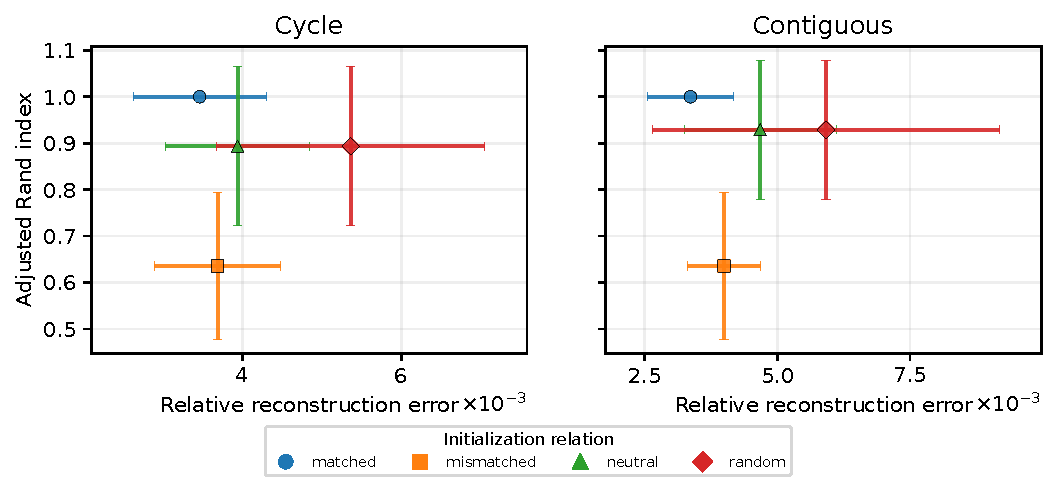
\includegraphics[width=.72\linewidth]{figures/factorization_loss_vs_ari.pdf}
  \caption{Soft-router exact-factorization runs for cycle and contiguous
  teachers.  Reconstruction error and planted-graph recovery are separate
  axes.}
  \label{fig:factorization}
\end{figure}
}{}

\IfFileExists{figures/distillation_loss_vs_ari.pdf}{%
\begin{figure}[H]
  \centering
  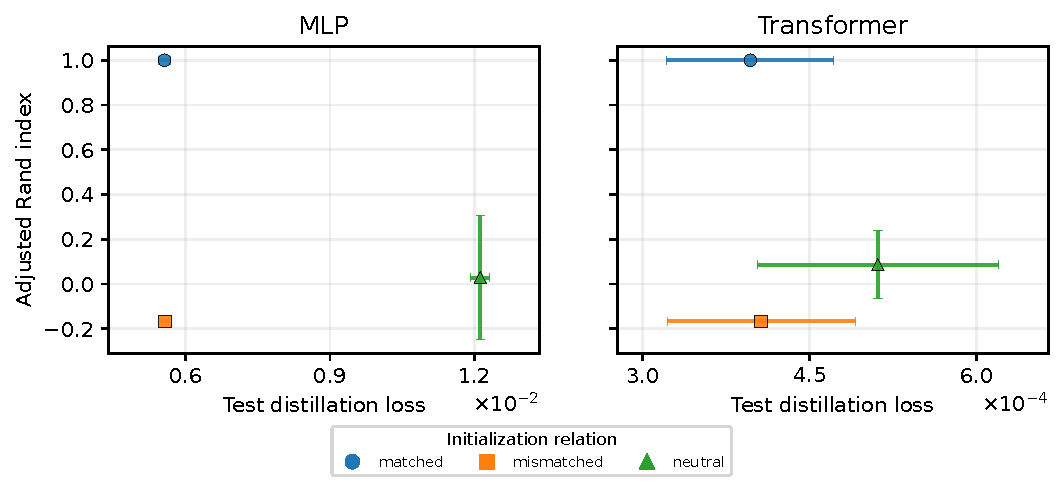
\includegraphics[width=.72\linewidth]{figures/distillation_loss_vs_ari.pdf}
  \caption{Distillation loss versus planted-graph ARI for the residual MLP and
  causal Transformer sanity checks.}
  \label{fig:distillation}
\end{figure}
}{}

\IfFileExists{generated/probe_table.tex}{% Auto-generated by experiments/analyze_results.py; do not edit by hand.
\begin{table}[H]
\centering
\small
\caption{Paired probe recovery aggregated over probe counts, fixed additive-noise levels, graphs, and seeds. Functional modes share inputs, noise, and projection. The visible-effective-parameter baseline uses neither observation noise nor projection and is not a test of functional equivalence. Values are mean $\pm$ sample standard deviation.}
\label{tab:probes}
\begin{tabular}{llrrr}
\toprule
Architecture & Signature & ARI & Empirical gap & $n$ \\
\midrule
MLP & shared input & $0.676 \pm 0.432$ & $-27.192 \pm 66.232$ & 1680 \\
MLP & native & $0.675 \pm 0.434$ & $-27.293 \pm 66.173$ & 1680 \\
MLP & effective parameter & $1.000 \pm 0$ & $0.008 \pm 5.82\!\times\!10^{-5}$ & 1680 \\
Transformer & shared input & $0.501 \pm 0.471$ & $-88.706 \pm 190.527$ & 1680 \\
Transformer & native & $0.501 \pm 0.470$ & $-88.758 \pm 190.490$ & 1680 \\
Transformer & effective parameter & $1.000 \pm 0$ & $0.009 \pm 2.08\!\times\!10^{-5}$ & 1680 \\
\bottomrule
\end{tabular}
\end{table}
}{}
\IfFileExists{figures/probe_phase_diagram.pdf}{%
\begin{figure}[H]
  \centering
  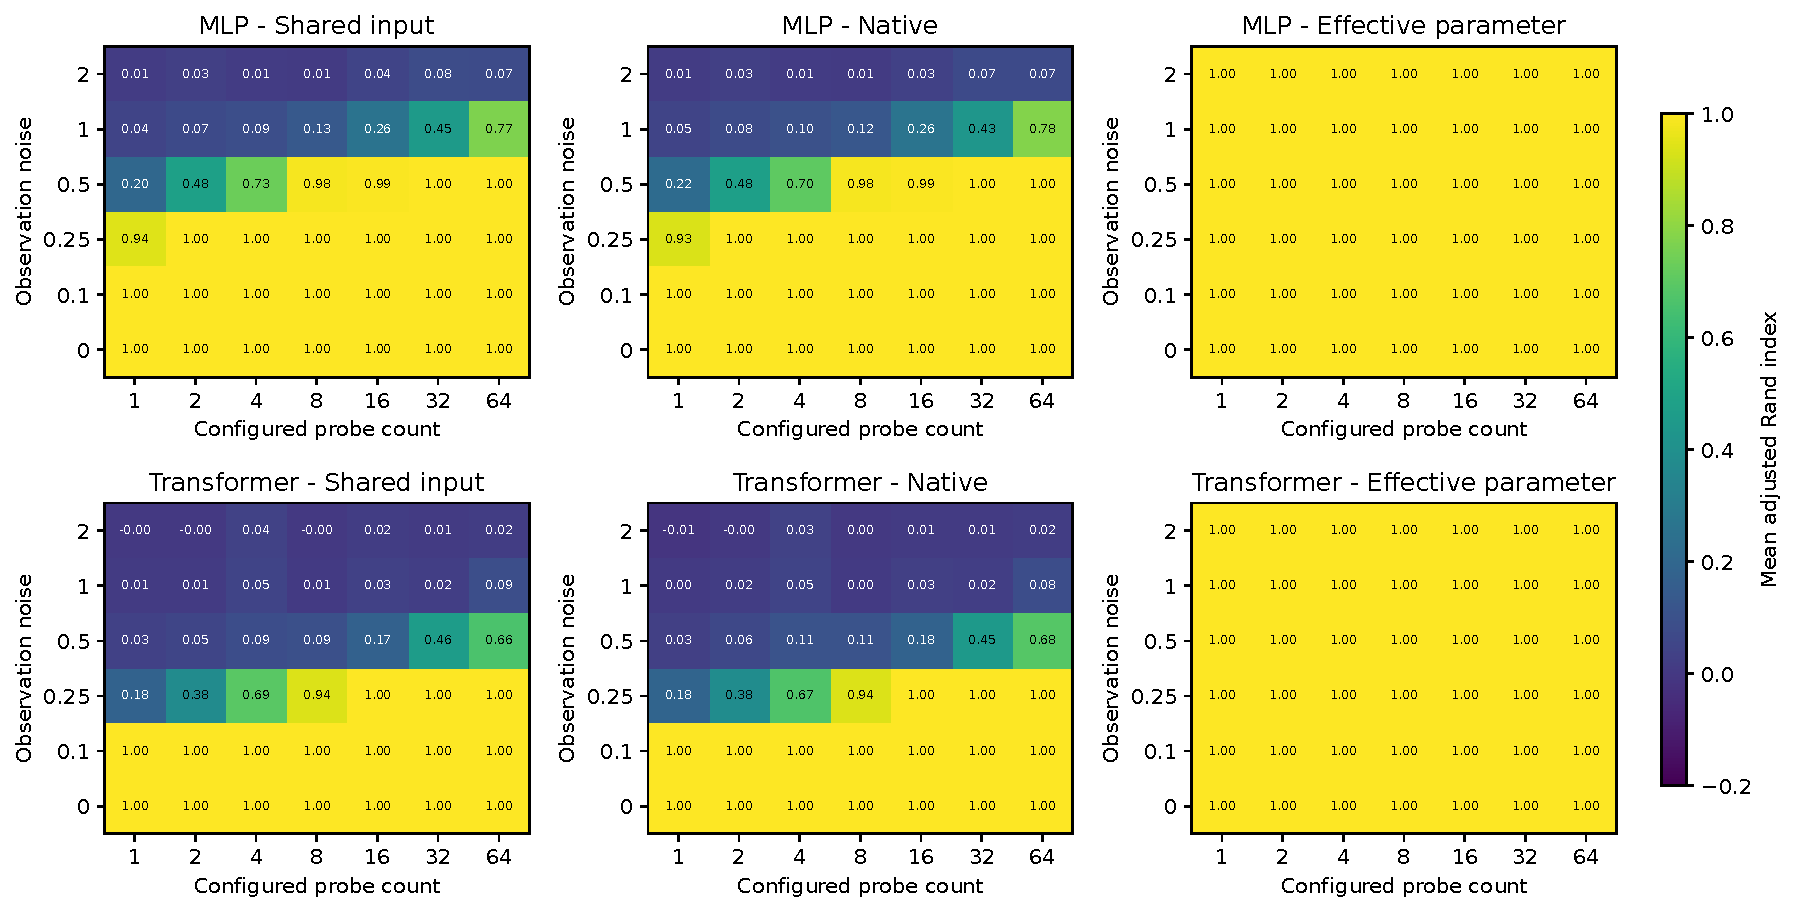
\includegraphics[width=.96\linewidth]{figures/probe_phase_diagram.pdf}
  \caption{Shared-input, native-signature, and visible-effective-parameter
  recovery as probe count and fixed additive observation noise vary.  The
  parameter baseline is repeated across the grid only for comparison and is
  not a functional-equivalence test.  This is a planted-partition sanity check,
  not evidence of superiority on natural systems.}
  \label{fig:probes}
\end{figure}
}{}

Functional-signature recovery generally improves with probe count and degrades
with observation noise.  The empirical within/between gap is computed against
the planted partition, rather than against the predicted clusters, but remains
only a finite-sample diagnostic unless the theorem's population gap and uniform
concentration assumptions are justified for this observation model.

\section{Language-model stability results}
\label{app:language-results}

\IfFileExists{generated/language_table.tex}{%
  % Auto-generated by experiments/analyze_results.py; do not edit by hand.
\begin{table}[H]
\centering
\small
\caption{Language-model stress test. BPB is estimated from 100 seeded, sampled test batches. Values are mean $\pm$ sample standard deviation across seeds; pairwise ARI descriptively summarizes the three dependent run pairs.}
\label{tab:language}
\begin{tabular}{lrrrr}
\toprule
Initialization & Sampled test BPB & L1 movement & Pairwise ARI & $n$ \\
\midrule
neutral & $2.415 \pm 0.009$ & $0.012 \pm 0.003$ & $0.099 \pm 0.157$ & 3 \\
pattern\_contiguous & $2.111 \pm 0.008$ & $3.10\!\times\!10^{-4} \pm 1.35\!\times\!10^{-5}$ & $1.000 \pm 0$ & 3 \\
pattern\_cycle & $2.181 \pm 0.011$ & $3.50\!\times\!10^{-4} \pm 4.60\!\times\!10^{-5}$ & $1.000 \pm 0$ & 3 \\
random & $2.319 \pm 0.015$ & $0.065 \pm 0.008$ & $-0.045 \pm 0.112$ & 3 \\
\bottomrule
\end{tabular}
\end{table}

}{The aggregate language-model table is generated by the analysis script.}

Distinct structured initializations can retain their partitions while reaching
competitive BPB.  With no privileged natural-language graph, this is evidence
of initialization dependence, not evidence that either retained partition is
false or historically correct.  The one-of-three partition-fold witness in
Table~\ref{tab:router-decision} is reported separately and does not convert this
stability arm into a prevalence result.

\section{Reproducibility checklist}

The response summary validates source hashes, checkpoint hashes, rank
assumptions, analytic/native formula agreement, the permutation control, and
all fixed probe outcomes.  The separate tomography summary validates three
newly generated raw artifacts, exact-gauge/common-design gates, rank and
dimension conditions, component reconstruction, and the permutation and
non-permutation controls without changing the older response generator.  The ASLoRA summary validates a common protocol hash,
generation-time source hashes, complete declared candidate coverage, the
canonical equivalence gate, and exact restoration for every seed and gauge.
The router-decision summary retains both exhausted searches, their full funnel
counts, checkpoint hashes, and the paired successful-seed evaluation; unlike
the other three summaries, it does not itself contain a generation-source-hash
attestation, so we do not claim equal provenance strength.

The artifact additionally includes deterministic seed handling, raw JSON
records, executable summarizers, the script that generates the three original audit
LaTeX tables and their appendix details from validated summaries, tests for summary-gate failures,
and unit tests for causal masking, permutation-invariant metrics, gauge
equivalence, response formulas, structured response reconstruction and its
approximate-product rejection boundary, restoration, and probe recovery.  Dataset
download is separated from training and accesses no private data.
